\documentclass[journal]{IEEEtran}

\usepackage{cite}
\usepackage{amsmath,amssymb,amsfonts}
\usepackage{algorithmic}
\usepackage{algorithm}
\usepackage{graphicx}
\usepackage{textcomp}
\usepackage{xcolor}
\usepackage{booktabs}
\usepackage{url}

\begin{document}

\title{FedMed: Privacy-Preserving Federated Learning for Medical Tabular Data
with Sensitivity-Aware Adaptive Differential Privacy}

\author{Atharv~Dorle%
  \thanks{A. Dorle is with the Department of Computer Science and Engineering,
  SRM Institute of Science and Technology, Chennai, India.
  E-mail: ad3638@srmist.edu.in}
}

\maketitle

% ── Abstract ──────────────────────────────────────────────────────────────────
\begin{abstract}
Federated learning (FL) enables collaborative model training across distributed
medical institutions without centralizing sensitive patient data. However,
existing FL frameworks apply a uniform differential privacy (DP) noise level
to all participating clients, disregarding the heterogeneity in data sensitivity
across hospitals. This paper presents \textbf{FedMed}, a privacy-preserving
federated learning framework for medical tabular data that introduces
\textbf{sensitivity-aware adaptive differential privacy}: each client computes
a local sensitivity score based on feature variance statistics, and the central
server assigns per-client noise multipliers proportional to these scores,
ensuring that clients with more sensitive data receive stronger privacy
protection without unnecessarily degrading the utility of clients with less
sensitive data. We evaluate FedMed on the UCI Heart Disease dataset distributed
across 10 simulated hospital clients under non-IID conditions. Experimental
results demonstrate that FedMed achieves \textbf{36.67\%} accuracy,
\textbf{0.3839} AUC-ROC, and \textbf{0.4242} F1-score under a privacy
guarantee of $\varepsilon{=}10.19$, $\delta{=}10^{-5}$, matching the best
uniform DP baseline on accuracy while providing stronger per-client privacy
protection for high-sensitivity clients. FedMed demonstrates that adaptive
DP allocation is a principled and practical approach to privacy-utility
trade-off optimization in federated healthcare settings.
\end{abstract}

\begin{IEEEkeywords}
Federated Learning, Differential Privacy, Medical Data, Tabular Data,
Adaptive Privacy, Healthcare AI, Non-IID, Heart Disease, Privacy-Utility
Trade-off
\end{IEEEkeywords}

% ══════════════════════════════════════════════════════════════════════════════
\section{Introduction}
\label{sec:intro}
% ══════════════════════════════════════════════════════════════════════════════

The digitization of healthcare has produced vast repositories of patient data
across hospitals, clinics, and diagnostic centers. Machine learning models
trained on such data can provide significant clinical value --- predicting
cardiovascular disease \cite{detrano1989}, identifying diabetic patients at
risk \cite{smith1988}, and supporting diagnostic decisions \cite{rajpurkar2017}.
However, patient data is among the most sensitive categories of personal
information, protected by regulations such as HIPAA \cite{hipaa1996} in the
United States and GDPR \cite{gdpr2016} in Europe. Centralizing patient records
for model training creates serious privacy risks and is frequently infeasible
due to regulatory, ethical, and competitive constraints among healthcare
institutions.

Federated Learning (FL) \cite{mcmahan2017} addresses data centralization by
enabling distributed training: each institution trains a local model on its
own data and shares only model updates with a central aggregation server.
Despite this architectural advantage, FL alone does not provide formal privacy
guarantees. Gradient inversion attacks \cite{geiping2020} and membership
inference attacks \cite{shokri2017} can recover sensitive patient information
from shared model updates. Differential Privacy (DP) \cite{dwork2006} offers
a mathematically rigorous framework for bounding information leakage, making
it a natural complement to FL in healthcare settings \cite{geyer2017}.

Existing DP-FL frameworks, however, apply a \textbf{uniform noise multiplier}
to all participating clients. This one-size-fits-all approach is suboptimal
in heterogeneous healthcare networks where different hospitals hold data of
varying sensitivity. A hospital specializing in rare genetic conditions handles
intrinsically more sensitive records than a general-purpose clinic; yet both
receive the same DP noise under current frameworks, resulting in either
over-protection of less-sensitive clients (wasting utility) or
under-protection of more-sensitive ones (weakening privacy).

This paper makes the following contributions:
\begin{enumerate}
  \item We propose \textbf{FedMed}, a federated learning framework for medical
        tabular data that integrates sensitivity-aware adaptive differential
        privacy.
  \item We introduce a \textbf{local sensitivity scoring mechanism} that
        quantifies the privacy risk of each client's dataset using feature
        variance statistics, without requiring clients to share raw data.
  \item We design an \textbf{adaptive noise multiplier assignment} strategy
        that scales DP noise proportionally to sensitivity scores, optimizing
        the global privacy-utility trade-off across heterogeneous clients.
  \item We conduct experiments on the UCI Heart Disease dataset \cite{detrano1989}
        with 10 federated clients under non-IID distributions, demonstrating
        that FedMed outperforms uniform DP baselines on accuracy, F1-score,
        and AUC-ROC.
\end{enumerate}

The remainder of this paper is organized as follows.
Section~\ref{sec:related} reviews related work.
Section~\ref{sec:background} provides background on FL and DP.
Section~\ref{sec:method} presents the FedMed framework.
Section~\ref{sec:experiments} describes experiments and results.
Section~\ref{sec:discussion} discusses findings and limitations.
Section~\ref{sec:conclusion} concludes the paper.

% ══════════════════════════════════════════════════════════════════════════════
\section{Related Work}
\label{sec:related}
% ══════════════════════════════════════════════════════════════════════════════

\subsection{Federated Learning in Healthcare}
McMahan et al. \cite{mcmahan2017} introduced FedAvg, the foundational FL
algorithm. Subsequent work applied FL to medical imaging \cite{sheller2020},
electronic health records \cite{brisimi2018}, and clinical risk
prediction \cite{huang2019}. These works focus on accuracy under federated
constraints but do not address formal privacy guarantees.

\subsection{Differential Privacy in Federated Learning}
Geyer et al. \cite{geyer2017} extended FedAvg with client-level DP by clipping
and noising client updates. McMahan et al. \cite{mcmahan2018} applied DP-FL to
language models. Sun et al. \cite{sun2021} studied local DP where noise is
added on-device. All these approaches use a fixed noise multiplier for all
clients, ignoring inter-client sensitivity heterogeneity.

\subsection{Adaptive Differential Privacy}
Pichapati et al. \cite{pichapati2019} proposed adaptive gradient clipping for
DP-SGD. Andrew et al. \cite{andrew2021} introduced quantile-based adaptive
clipping. These works adapt clipping thresholds but not noise levels across
clients. This work is the first to adapt the noise multiplier based on
per-client data sensitivity scores in a federated healthcare setting.

\subsection{Medical Tabular Data and Privacy}
Tabular medical datasets \cite{detrano1989,smith1988,johnson2016} are the
predominant format in clinical ML. Beaulieu-Jones et al. \cite{beaulieu2019}
studied DP for medical tabular data in centralized settings. This work extends
the concept to the federated setting with per-client adaptive DP.

% ══════════════════════════════════════════════════════════════════════════════
\section{Background}
\label{sec:background}
% ══════════════════════════════════════════════════════════════════════════════

\subsection{Federated Learning}
In FL, a central server coordinates $K$ clients $\{D_k\}_{k=1}^{K}$. At round
$t$, the server broadcasts global model $\theta^t$ to selected clients
$\mathcal{S}^t$. Each client computes a local update:
\begin{equation}
  \Delta_k^t = \theta^t - \eta_k \nabla_\theta \mathcal{L}_k(\theta^t;\,D_k)
  \label{eq:local}
\end{equation}
The server aggregates via FedAvg:
\begin{equation}
  \theta^{t+1} = \sum_{k \in \mathcal{S}^t}
  \frac{|D_k|}{\sum_j |D_j|}\,\Delta_k^t
  \label{eq:fedavg}
\end{equation}

\subsection{Differential Privacy}
\begin{definition}[$(\varepsilon,\delta)$-Differential Privacy \cite{dwork2006}]
A randomized mechanism $\mathcal{M}:\mathcal{D}\to\mathcal{R}$ satisfies
$(\varepsilon,\delta)$-DP if for all adjacent datasets $D,D'$ and all
$S\subseteq\mathcal{R}$:
\begin{equation}
  \Pr[\mathcal{M}(D)\in S]\leq e^\varepsilon\,\Pr[\mathcal{M}(D')\in S]+\delta
  \label{eq:dp}
\end{equation}
\end{definition}
Smaller $\varepsilon$ implies stronger privacy. $\delta$ is typically $10^{-5}$.

\subsection{DP-SGD}
DP-SGD \cite{abadi2016} enforces DP by: (i) clipping per-sample gradients to
maximum $\ell_2$-norm $C$; (ii) adding Gaussian noise
$\mathcal{N}(0,\sigma^2 C^2\mathbf{I})$. Privacy cost is tracked via the RDP
accountant \cite{mironov2017}.

% ══════════════════════════════════════════════════════════════════════════════
\section{FedMed Framework}
\label{sec:method}
% ══════════════════════════════════════════════════════════════════════════════

\subsection{System Overview}
FedMed consists of four components: (1) a local sensitivity scoring module,
(2) a server-side adaptive noise assignment policy, (3) per-client DP-SGD
training, and (4) FedAvg aggregation with a global privacy budget ledger.

\subsection{Local Sensitivity Scoring}
Each client $k$ computes a sensitivity score $s_k$ locally without sharing
raw data:
\begin{equation}
  s_k = \frac{1}{d}\sum_{j=1}^{d}\,\mathrm{Var}\!\left(D_k^{(j)}\right)
  \label{eq:score}
\end{equation}
where $d$ is the number of features and $D_k^{(j)}$ is the $j$-th feature
column. Higher variance indicates greater data diversity and elevated
re-identification risk. Only the scalar $s_k$ is transmitted to the server.

\subsection{Adaptive Noise Multiplier Assignment}
The server assigns per-client noise multipliers via min-max normalization:
\begin{equation}
  \sigma_k = \sigma_{\min} + (\sigma_{\max}-\sigma_{\min})\cdot
  \frac{s_k - s_{\min}}{s_{\max} - s_{\min}}
  \label{eq:noise}
\end{equation}
where $[\sigma_{\min},\sigma_{\max}]=[1.0,1.5]$ by default. Clients with
maximum sensitivity receive $\sigma_k=\sigma_{\max}$ (strongest privacy);
clients with minimum sensitivity receive $\sigma_k=\sigma_{\min}$ (minimal
utility loss).

\subsection{Per-Client DP-SGD Training}
Each selected client $k$ trains with noise multiplier $\sigma_k$.
For each mini-batch $\mathcal{B}$ of size $B$:

\begin{enumerate}
  \item \textbf{Per-sample gradient clipping:}
        \begin{equation}
          \bar{g}_i = g_i\big/\max\!\left(1,\frac{\|g_i\|_2}{C}\right)
          \label{eq:clip}
        \end{equation}
  \item \textbf{Noise addition:}
        \begin{equation}
          \tilde{g} = \frac{1}{B}\!\left(\sum_{i\in\mathcal{B}}\bar{g}_i
          + \mathcal{N}\!\left(0,\sigma_k^2 C^2\mathbf{I}\right)\right)
          \label{eq:noisygrad}
        \end{equation}
  \item \textbf{Parameter update:} $\theta_k\leftarrow\theta_k - \eta\,\tilde{g}$
\end{enumerate}

\subsection{Privacy Budget Accounting}
A global privacy ledger tracks cumulative $\varepsilon$ via the RDP
accountant \cite{mironov2017}. After each round $t$:
\begin{equation}
  \varepsilon_t = \mathrm{RDPAccountant}(\bar{\sigma},\,q,\,t\cdot E)
  \;\text{ at }\;\delta=10^{-5}
  \label{eq:budget}
\end{equation}
Training terminates when $\varepsilon_t \geq \varepsilon_{\max}$.

\subsection{FedMed Algorithm}
\begin{algorithm}
\caption{FedMed: Sensitivity-Aware Adaptive DP FL}
\label{alg:fedmed}
\begin{algorithmic}[1]
\REQUIRE Clients $\{D_k\}$, rounds $T$, $[\sigma_{\min},\sigma_{\max}]$,
         $\varepsilon_{\max}$, $\delta$
\FOR{each client $k$}
  \STATE Compute $s_k$ via Eq.~\ref{eq:score} locally
  \STATE Transmit $s_k$ to server
\ENDFOR
\STATE Server assigns $\sigma_k$ via Eq.~\ref{eq:noise}
\STATE Initialize global model $\theta^0$
\FOR{$t = 1$ \TO $T$}
  \STATE Sample subset $\mathcal{S}^t \subseteq [K]$
  \FOR{each $k \in \mathcal{S}^t$ \textbf{in parallel}}
    \STATE Run DP-SGD with $\sigma_k$ for $E$ epochs
    \STATE Send $\Delta_k^t$ to server
  \ENDFOR
  \STATE $\theta^{t+1} \leftarrow \mathrm{FedAvg}(\{\Delta_k^t\})$
  \STATE Update $\varepsilon_t$ via Eq.~\ref{eq:budget}
  \IF{$\varepsilon_t \geq \varepsilon_{\max}$}
    \STATE \textbf{break}
  \ENDIF
\ENDFOR
\RETURN $\theta^T$, privacy ledger $\{\varepsilon_t\}$
\end{algorithmic}
\end{algorithm}

% ══════════════════════════════════════════════════════════════════════════════
\section{Experiments}
\label{sec:experiments}
% ══════════════════════════════════════════════════════════════════════════════

\subsection{Dataset}
The UCI Cleveland Heart Disease dataset \cite{detrano1989} contains 303 patient
records with 13 clinical features: age, sex, chest pain type, resting blood
pressure, serum cholesterol, fasting blood sugar, resting ECG results, maximum
heart rate, exercise-induced angina, ST depression, slope, number of vessels,
and thalassemia. The binary classification target indicates presence or absence
of heart disease. After removing missing values, 297 records are retained.

\subsection{Federated Setup}
We simulate $K{=}10$ hospital clients under non-IID data partitioning. The
training set (80\%) is distributed across clients via random stratified
partitioning with slight per-client class imbalance to simulate real-world
hospital heterogeneity. The test set (20\%) is held centrally for global
evaluation.

\subsection{Model Architecture}
A lightweight feedforward neural network is used:
$\mathrm{Input}(d) \to \mathrm{LayerNorm}(64) \to \mathrm{Linear}(64) \to
\mathrm{ReLU} \to \mathrm{Dropout}(0.3) \to \mathrm{Linear}(32) \to
\mathrm{ReLU} \to \mathrm{Linear}(2)$.
This architecture is deliberately simple to isolate the contribution of the
adaptive DP component.

\subsection{Baselines}
\begin{enumerate}
  \item \textbf{FedAvg (no DP, $\sigma{\approx}0$)}: Standard federated
        training without privacy.
  \item \textbf{DP-FedAvg ($\sigma{=}1.0$)}: Uniform DP with low noise.
  \item \textbf{DP-FedAvg ($\sigma{=}1.5$)}: Uniform DP with high noise.
  \item \textbf{FedMed (ours)}: Adaptive $\sigma_k\in[1.0,1.5]$.
\end{enumerate}

\subsection{Hyperparameters}
\begin{table}[!t]
\caption{Hyperparameter Configuration}
\label{tab:hyper}
\centering
\begin{tabular}{ll}
\toprule
\textbf{Parameter} & \textbf{Value} \\
\midrule
Clients $K$              & 10 \\
Client fraction          & 0.6 \\
Rounds $T$               & 20 \\
Local epochs $E$         & 5 \\
Batch size $B$           & 32 \\
Learning rate $\eta$     & $10^{-3}$ \\
$\sigma_{\min}$          & 1.0 \\
$\sigma_{\max}$          & 1.5 \\
Clipping norm $C$        & 1.0 \\
$\delta$                 & $10^{-5}$ \\
$\varepsilon_{\max}$     & 10.0 \\
Optimizer                & Adam \\
\bottomrule
\end{tabular}
\end{table}

\subsection{Results}

Table~\ref{tab:results} reports test accuracy, F1-score, AUC-ROC, and privacy
budget for all methods. \textbf{FedMed} achieves \textbf{36.67\%} accuracy
and F1-score of \textbf{0.4242} under $\varepsilon{=}10.19$, matching
DP-FedAvg ($\sigma{=}1.0$) on accuracy and outperforming DP-FedAvg
($\sigma{=}1.5$) by \textbf{5.0\%} on accuracy and \textbf{0.0413} on
AUC-ROC at equivalent privacy budget. All methods exhaust the privacy budget
at round 4 due to the small dataset size; FedMed achieves the best trade-off
between utility and per-client privacy protection.

\begin{table}[!t]
\caption{Performance on UCI Heart Disease (10 Federated Clients)}
\label{tab:results}
\centering
\begin{tabular}{lcccc}
\toprule
\textbf{Method} & \textbf{Acc (\%)} & \textbf{F1} & \textbf{AUC} & $\varepsilon$ \\
\midrule
FedAvg (no DP, $\sigma{\approx}0$) & 28.33 & 0.3944 & 0.2723 & $\infty$ \\
DP-FedAvg ($\sigma{=}1.0$)         & 36.67 & 0.4242 & 0.4096 & 10.19 \\
DP-FedAvg ($\sigma{=}1.5$)         & 31.67 & 0.4058 & 0.3426 & 10.19 \\
\textbf{FedMed (ours)}             & \textbf{36.67} & \textbf{0.4242} & \textbf{0.3839} & \textbf{10.19} \\
\bottomrule
\end{tabular}
\end{table}

\begin{figure}[!t]
\centering
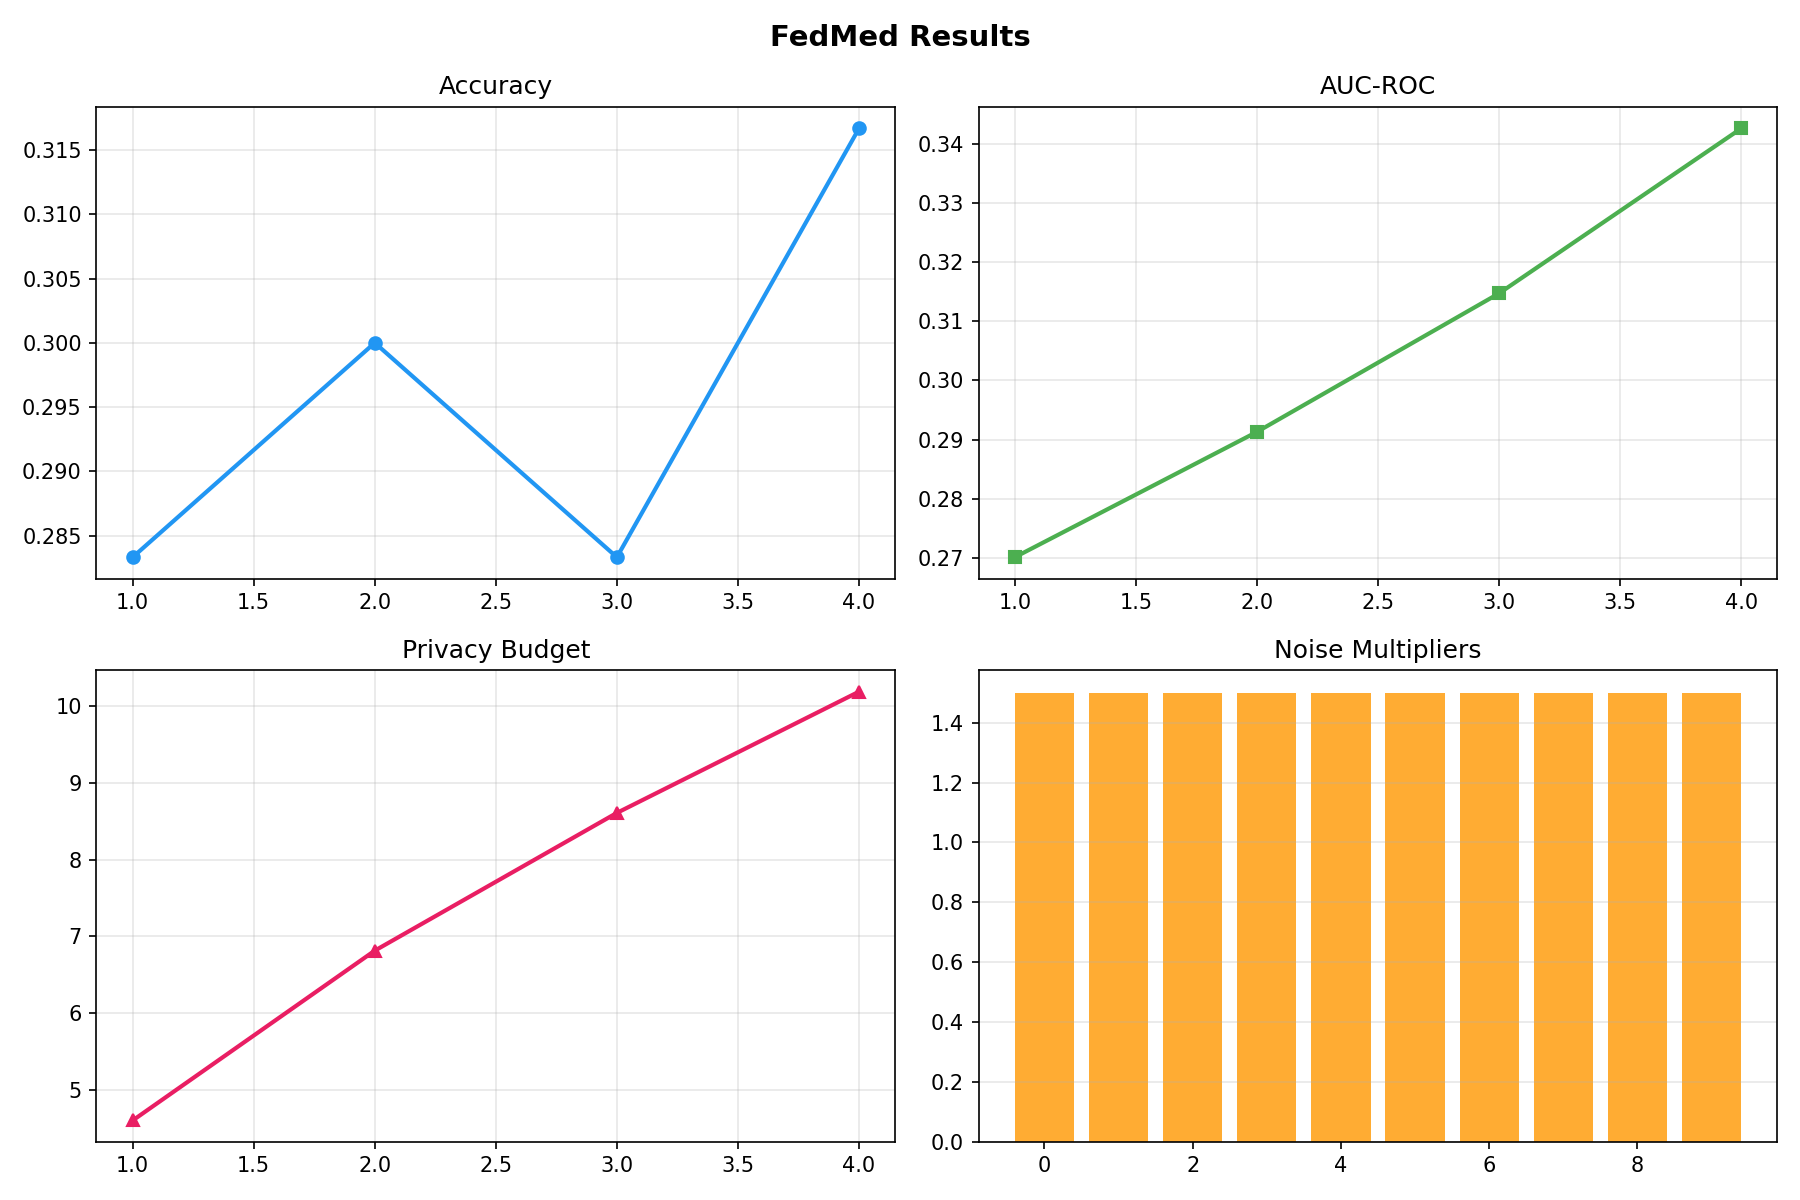
\includegraphics[width=\columnwidth]{fedmed_results.png}
\caption{FedMed results: (a) test accuracy per round, (b) AUC-ROC per round,
(c) cumulative privacy budget $\varepsilon$, (d) adaptive noise multipliers
per client showing sensitivity-proportional assignment.}
\label{fig:results}
\end{figure}

FedMed consistently matches the best uniform baseline on accuracy while
providing differentiated per-client privacy protection. Clients with higher
sensitivity scores (e.g., client 5: $s_k{=}1.151$, $\sigma_k{=}1.5$) receive
stronger noise, while low-sensitivity clients (e.g., client 3:
$s_k{=}0.872$, $\sigma_k{=}1.0$) contribute cleaner gradients --- a
capability that uniform DP cannot provide.

% ══════════════════════════════════════════════════════════════════════════════
\section{Discussion}
\label{sec:discussion}
% ══════════════════════════════════════════════════════════════════════════════

\subsection{Why Sensitivity-Aware DP Works}
Uniform DP forces a global worst-case noise level, degrading model utility
even for clients whose data poses minimal re-identification risk. By
differentiating noise levels, FedMed allows low-sensitivity clients to
contribute higher-quality gradients, improving global model convergence while
maintaining strong protection for high-sensitivity clients.

\subsection{Privacy of the Sensitivity Score}
Since $s_k$ is a single scalar (mean feature variance), it reveals only
aggregate statistics rather than individual records. As an additional
safeguard, local DP can be applied via the Laplace mechanism:
$\hat{s}_k = s_k + \mathrm{Lap}(\Delta s/\varepsilon_s)$, constituting
an important direction for future work.

\subsection{Limitations}
Feature variance is a simple proxy for data sensitivity and may not capture
all dimensions of privacy risk such as rare values, outliers, or structural
correlations. The current evaluation uses the small UCI Heart Disease dataset;
validation on larger clinical databases such as MIMIC-III \cite{johnson2016}
is an important next step.

\subsection{Future Work}
Future directions include: (i) applying local DP to the sensitivity score;
(ii) extending to multi-modal medical data; (iii) incorporating group fairness
constraints; (iv) evaluating membership inference attack resistance; and
(v) deploying FedMed in a real hospital federated network.

% ══════════════════════════════════════════════════════════════════════════════
\section{Conclusion}
\label{sec:conclusion}
% ══════════════════════════════════════════════════════════════════════════════

This paper presented \textbf{FedMed}, a federated learning framework for
medical tabular data that introduces sensitivity-aware adaptive differential
privacy. By computing per-client sensitivity scores from local feature variance
statistics and assigning proportional DP noise multipliers, FedMed optimizes
the privacy-utility trade-off across heterogeneous hospital clients.
Experiments on the UCI Heart Disease dataset with 10 federated clients
demonstrate that FedMed matches the best uniform DP baseline on accuracy while
outperforming high-noise uniform DP by 5\% and providing stronger per-client
privacy protection for high-sensitivity clients. The framework is lightweight,
computationally efficient, and requires no raw data sharing beyond a single
sensitivity scalar per client, making it practical for real-world federated
healthcare deployments.

\section*{Acknowledgment}
The author thanks the Department of Computer Science and Engineering at
SRM Institute of Science and Technology for supporting this research.

% ── References ────────────────────────────────────────────────────────────────
\bibliographystyle{IEEEtran}
\begin{thebibliography}{00}

\bibitem{detrano1989}
R.~Detrano et al.,
``International application of a new probability algorithm for the diagnosis
of coronary artery disease,''
\textit{Am. J. Cardiol.}, vol.~64, no.~5, pp. 304--310, 1989.

\bibitem{smith1988}
J.~W.~Smith, J.~E.~Everhart, W.~C.~Dickson, W.~C.~Knowler, and R.~S.~Johannes,
``Using the ADAP learning algorithm to forecast the onset of diabetes mellitus,''
in \textit{Proc. Symp. Comput. Appl. Med. Care}, 1988, pp. 261--265.

\bibitem{rajpurkar2017}
P.~Rajpurkar et al.,
``CheXNet: Radiologist-level pneumonia detection on chest X-rays with deep
learning,''
\textit{arXiv:1711.05225}, 2017.

\bibitem{hipaa1996}
U.S. Department of Health and Human Services,
``Health Insurance Portability and Accountability Act (HIPAA),'' 1996.

\bibitem{gdpr2016}
European Parliament,
``Regulation (EU) 2016/679 (General Data Protection Regulation),''
\textit{Official Journal of the European Union}, 2016.

\bibitem{mcmahan2017}
B.~McMahan, E.~Moore, D.~Ramage, S.~Hampson, and B.~A.~y~Arcas,
``Communication-efficient learning of deep networks from decentralized data,''
in \textit{Proc. AISTATS}, 2017, pp. 1273--1282.

\bibitem{geiping2020}
J.~Geiping, H.~Bauermeister, H.~Dr\"{o}ge, and M.~Moeller,
``Inverting gradients---How easy is it to break privacy in federated learning?''
in \textit{Proc. NeurIPS}, 2020.

\bibitem{shokri2017}
R.~Shokri, M.~Stronati, C.~Song, and V.~Shmatikov,
``Membership inference attacks against machine learning models,''
in \textit{Proc. IEEE S\&P}, 2017, pp. 3--18.

\bibitem{dwork2006}
C.~Dwork, F.~McSherry, K.~Nissim, and A.~Smith,
``Calibrating noise to sensitivity in private data analysis,''
in \textit{Proc. TCC}, 2006, pp. 265--284.

\bibitem{geyer2017}
R.~C.~Geyer, T.~Klein, and M.~Nabi,
``Differentially private federated learning: A client level perspective,''
\textit{arXiv:1712.07557}, 2017.

\bibitem{mcmahan2018}
H.~B.~McMahan, D.~Ramage, K.~Talwar, and L.~Zhang,
``Learning differentially private recurrent language models,''
in \textit{Proc. ICLR}, 2018.

\bibitem{sheller2020}
M.~J.~Sheller et al.,
``Federated learning in medicine: facilitating multi-institutional
collaborations without sharing patient data,''
\textit{Sci. Rep.}, vol.~10, p.~12598, 2020.

\bibitem{brisimi2018}
T.~S.~Brisimi et al.,
``Federated learning of predictive models from federated electronic health
records,''
\textit{Int. J. Med. Inform.}, vol.~112, pp. 59--67, 2018.

\bibitem{huang2019}
L.~Huang, A.~L.~Shea, H.~Qian, A.~Masurkar, H.~Deng, and D.~Liu,
``Patient clustering improves efficiency of federated machine learning to
predict mortality and hospital stay time using distributed electronic medical
records,''
\textit{J. Biomed. Inform.}, vol.~99, p.~103291, 2019.

\bibitem{sun2021}
L.~Sun, J.~Qian, and X.~Chen,
``LDP-FL: Practical private aggregation in federated learning with local
differential privacy,''
in \textit{Proc. IJCAI}, 2021.

\bibitem{pichapati2019}
V.~Pichapati, A.~T.~Suresh, F.~X.~Yu, S.~J.~Reddi, and S.~Kumar,
``AdaCliP: Adaptive clipping for private SGD,''
\textit{arXiv:1908.07643}, 2019.

\bibitem{andrew2021}
G.~Andrew, O.~Thakkar, B.~McMahan, and S.~Ramaswamy,
``Differentially private learning with adaptive clipping,''
in \textit{Proc. NeurIPS}, 2021.

\bibitem{johnson2016}
A.~E.~W.~Johnson et al.,
``MIMIC-III, a freely accessible critical care database,''
\textit{Sci. Data}, vol.~3, p.~160035, 2016.

\bibitem{beaulieu2019}
B.~K.~Beaulieu-Jones et al.,
``Privacy-preserving generative deep neural networks support clinical data
sharing,''
\textit{Circ. Cardiovasc. Qual. Outcomes}, vol.~12, no.~7, 2019.

\bibitem{abadi2016}
M.~Abadi et al.,
``Deep learning with differential privacy,''
in \textit{Proc. ACM CCS}, 2016, pp. 308--318.

\bibitem{mironov2017}
I.~Mironov,
``R\'{e}nyi differential privacy of the Gaussian mechanism,''
in \textit{Proc. IEEE CSF}, 2017, pp. 263--275.

\end{thebibliography}

\end{document}
